\documentclass[a4paper]{article}
%\documentclass[a4paper,fontsize=13pt]{scrartcl}
\usepackage{vntex}
%\usepackage{helvet} %set font Helvetica
%\usepackage{times} %set font Times New Roman
\renewcommand{\familydefault}{\sfdefault} %set font Sans Serif

%%%%% change language vietname - english
%\usepackage[english,vietnam]{babel}
%\usepackage[utf8]{inputenc}
%\usepackage[francais]{babel}

\usepackage{a4wide,amssymb,epsfig,latexsym,array,hhline,fancyhdr}
\usepackage{amsmath}
\usepackage{amsthm}
\usepackage{multicol,longtable,amscd}
\usepackage{diagbox} %Make diagonal lines in tables
\usepackage{booktabs}
\usepackage{alltt}
\usepackage[framemethod=tikz]{mdframed} % For highlighting paragraph backgrounds
\usepackage{caption,subcaption}
\usepackage{lastpage}
\usepackage[lined,boxed,commentsnumbered]{algorithm2e}
\usepackage{enumerate}
\usepackage{color}
\usepackage{graphicx} % Standard graphics package
\usepackage{array}
\usepackage{tabularx, caption}
\usepackage{multirow}
\usepackage{rotating}
\usepackage{graphics}
\usepackage[left=2.5cm,right=2.5cm,top=2cm,bottom=3cm]{geometry} % margin page
\usepackage{a4wide,amssymb,epsfig,latexsym,array,hhline,fancyhdr}
\usepackage[makeroom]{cancel}
\usepackage{arydshln}
\usepackage{textcomp}
\usepackage{listings}
\usepackage{listingsutf8}
\usepackage{verbatim}
\usepackage{setspace}

\usepackage{epsfig}
\usepackage{tikz}
\usetikzlibrary{calc}
\newcommand\HRule{\rule{\textwidth}{1pt}}
\usetikzlibrary{arrows,snakes,backgrounds}
\usepackage[unicode]{hyperref}
\hypersetup{urlcolor=blue,linkcolor=black,citecolor=black,colorlinks=true} 
%\usepackage{pstcol} % PSTricks with the standard color package

\setlength\dashlinedash{1.5pt}
\setlength\dashlinegap{4.5pt}
\setlength\arrayrulewidth{0.2pt}

% Typesetting Listings
\usepackage{xcolor}
\usepackage{color}
\definecolor{listinggray}{gray}{0.9}
\definecolor{lbcolor}{rgb}{0.9,0.9,0.9}
\definecolor{Darkgreen}{rgb}{0.1,0.6,0.1}
\definecolor{whitesmoke}{rgb}{0.99, 0.99,0.99}

\lstset{
	backgroundcolor=\color{whitesmoke},
	tabsize=2,
	language=[GNU]C++,
	basicstyle=\scriptsize,
	upquote=true,
	aboveskip={1.5\baselineskip},
	columns=fixed,
	showstringspaces=false,
	extendedchars=false,
	breaklines=true,
	prebreak = \raisebox{0ex}[0ex][0ex]{\ensuremath{\hookleftarrow}},
	frame=single,
	numbers=left,
	showtabs=false,
	showspaces=false,
	showstringspaces=false,
	identifierstyle=\ttfamily,	
	keywordstyle=\color[rgb]{0,0,1},
	commentstyle=\color[rgb]{0.026,0.112,0.095},
	stringstyle=\color[rgb]{0.627,0.126,0.941},
	numberstyle=\color[rgb]{0.205, 0.142, 0.73},
	%\lstdefinestyle{C++}{language=C++,style=numbers}’.
}
\lstset{
	backgroundcolor=\color{whitesmoke},
	tabsize=2,
	language=C++,
	captionpos=b,
	frame=lines,
	numbers=left,
	numberstyle=\tiny,
	numbersep=5pt,
	breaklines=true,
	showstringspaces=false,
	basicstyle=\footnotesize,
	%identifierstyle=\color{magenta},
	keywordstyle=\color[rgb]{0,0,1},
	commentstyle=\color{Darkgreen},
	stringstyle=\color{red}
}

\setlength{\headheight}{40pt}
\pagestyle{fancy}
\fancyhead{} % clear all header fields
\fancyhead[L]{
	\begin{tabular}{rl}
		\begin{tabular}{l}
			\textbf{Ho Chi Minh University of Technology - 
				Faculty of Computer Science \& Engineering}\\
		\end{tabular} 	
	\end{tabular}
}
\fancyhead[R]{
	\begin{tabular}{l}
		\tiny \bf \\
		\tiny \bf 
\end{tabular}  }
\fancyfoot{} % clear all footer fields
\fancyfoot[L]{\footnotesize THỰC TẬP ĐỒ ÁN ĐA NGÀNH - BÁO CÁO NỘI DUNG 1 }
\fancyfoot[R]{\footnotesize Trang {\thepage}/\pageref{LastPage}}
\renewcommand{\headrulewidth}{0.1pt}
\renewcommand{\footrulewidth}{0.1pt}

\setcounter{secnumdepth}{4}
\setcounter{tocdepth}{3}
\makeatletter
\newcounter {subsubsubsection}[subsubsection]
\renewcommand\thesubsubsubsection{\thesubsubsection .\@alph\c@subsubsubsection}
\newcommand\subsubsubsection{\@startsection{subsubsubsection}{4}{\z@}%
	{-3.25ex\@plus -1ex \@minus -.2ex}%
	{1.5ex \@plus .2ex}%
	{\normalfont\normalsize\bfseries}}
\newcommand*\l@subsubsubsection{\@dottedtocline{3}{10.0em}{4.1em}}
\newcommand*{\subsubsubsectionmark}[1]{}
\makeatother

\everymath{\color{black}} %make in-line maths symbols blue to read/check easily

\sloppy
\captionsetup[figure]{labelfont={small,bf},textfont={small,it},belowskip=-1pt,aboveskip=-9pt}
%space remove between caption, figure, and text
\captionsetup[table]{labelfont={small,bf},textfont={small,it},belowskip=-1pt,aboveskip=7pt}
\setlength{\floatsep}{5pt plus 2pt minus 2pt}
\setlength{\textfloatsep}{5pt plus 2pt minus 2pt}
\setlength{\intextsep}{10pt plus 2pt minus 2pt}
\begin{document}
\begin{titlepage}

\begin{tikzpicture}[remember picture, overlay]
  \draw[line width = 3pt,color=blue] ($(current page.north west) + (2.2cm,-2.2cm)$) rectangle ($(current page.south east) + (-2.2cm,2.2cm)$);
   \draw[line width = 2pt,color=green] ($(current page.north west) + (2cm,-2cm)$) rectangle ($(current page.south east) + (-2cm,2cm)$);
\end{tikzpicture}
\vspace{1.5cm}
\begin{center} \large
ĐẠI HỌC BÁCH KHOA - ĐẠI HỌC QUỐC GIA THÀNH PHỐ HỒ CHÍ MINH \\
\textbf{KHOA KHOA HỌC VÀ KỸ THUẬT MÁY TÍNH} \\
- - - - - - - - - - - - - - - - - - - - - 
\end{center}


\vspace{1cm}
\begin{figure}[h!]
\begin{center}

\includegraphics[width=3.6cm]{Images/LogoBK}
\end{center}
\end{figure}
\vspace{1cm}



\begin{center}
\begin{tabular}{c}
\multicolumn{1}{c}{\textbf{{\Huge THỰC TẬP ĐỒ ÁN ĐA NGÀNH}}}\\
\\ \hline \\
\textbf{{\Large BÁO CÁO NỘI DUNG 2}}\\
\\
\textbf{{\large Phát triển hệ thống theo dõi nhiệt độ và độ ẩm các phòng trong  }}\\
\textbf{{\large một toà nhà, bật tắt thiết bị điều hoà/quạt khi nhiệt độ quá ngưỡng cho phép. }}\\
\textbf{{\large Ghi nhận hoạt động}}\\
\\ \hline \\
\end{tabular}
\end{center}
	\begin{table}[h]
	\begin{tabular}{rrlrr}
		\hspace{5cm} 
		& {\large Giảng viên hướng dẫn}: & {\large Trần Thị Quế Nguyệt} & & \\
		& {\large Nhóm}: & {\large 7} & & \\
		& {\large Sinh viên}: & {\large 1711929 - Ngô Thanh Liêm } \\
		& {} & {\large 1710188 - Cao Nguyệt Minh } \\
		& {} & {\large 1711830 - Đinh Vĩnh Khương } \\
		& {} & {\large 1711130 - Võ Quý Giang} \\
	\end{tabular}
\end{table}

\vspace{3cm}

\begin{center}
{\footnotesize Thành phố Hồ Chí Minh, 5/2020}
\end{center}

\end{titlepage}


\newpage \thispagestyle{empty} \tableofcontents
%\newpage \thispagestyle{empty} \listoftables
\newpage \thispagestyle{empty} \listoffigures

\newpage

%%%%%%%%%%%%%%%%%%%%%%%%%%%%%%%%%%%%%%%%%%%
% set noindent all document
\setlength{\parindent}{1cm}
%%%%%%%%%%%%%%%%%%%%%%%%%%%%%%%%%%%%%%%%%%%

\section{Tìm hiểu công nghệ và MQTT Server}

\subsection{Công nghệ sử dụng trong mobile app}
\subsubsection{React Native là gì?}
$\indent$
\textbf{React Native} là một framework do công ty công nghệ nổi tiếng Facebook phát triển, cho phép sử dụng JavaScript để làm ứng dụng, nhằm mục đích giải quyết bài toán hiệu năng của Hybrid và bài toán chi phí khi mà phải viết nhiều loại ngôn ngữ native cho từng nền tảng di động. \\
$\indent$
Chúng ta sẽ build được ứng dụng Native, và chúng ta cũng có thể build ứng dụng đó một cách đa nền tảng (multi-platform) chứ không phải là một “mobile web app”, không phải là “HTML5 app”, và cũng không phải là một “hybrid app” hay cũng không chỉ build trên iOS hay Android mà chúng ta build và chạy được cả hai hệ sinh thái.\\
$\indent$
Một điểm hay nữa mà React Native có là giảm chi phí recompile của Native bằng cách sử dụng Hot-Loading, có nghĩa là bạn không cần phải build lại ứng dụng từ đầu nên việc chỉnh sửa diễn ra rất nhanh chóng. Giúp cho lập trình viên có thể thấy được những chỉnh sửa của họ một cách nhanh chóng trực quan, không còn phải bỏ quá nhiều thời gian trong việc build và run ứng dụng nữa.\\
$\indent$
Và điểm lợi hại kế tiếp của React Native đó chính là chúng ta chỉ cần sử dụng JS (JavaScript) để phát triển được một ứng dụng di động hoàn chỉnh, đồng thời giải quyết được các vấn đề mà Native App gặp phải mà mình đã nêu ở trên. Và rồi còn cả kết hợp với code native như Swift, Java, v.v… \\ \\

\includegraphics[width=\columnwidth]{Images/reactnative}
\subsubsection{Cách hoạt động của React Native}
$\indent$
Bằng cách tích hợp 2 thread là \textbf{Main Thread} và \textbf{JS Thread} cho ứng dụng mobile. 
Với \textbf{Main Thread} sẽ đảm nhận vai trò cập nhật giao diện người dùng (UI). Sau đó sẽ xử lý tương tác người dùng. Trong khi đó, \textbf{JS Thread} sẽ thực thi và xử lý code Javascript. Hai luồng này hoạt động độc lập với nhau. \\
$\indent$
Để tương tác được với nhau hai Thread sẽ sử dụng một Bridge (cầu nối). Cho phép chúng giao tiếp mà không phụ thuộc lẫn nhau, chuyển đổi dữ liệu từ thread này sang thread khác. Dữ liệu từ hai Thread được vận hành khi tiếp nối dữ liệu cho nhau.

\subsection{MQTT Server}
\subsubsection{MQTT là gì?}
$\indent$
\textbf{MQTT (Message Queue Telemetry Transport)} là một giao thức truyền thông điệp (message) theo mô hình \textbf{Publish/Subscribe} (Xuất bản - Theo dõi), sử dụng băng thông thấp, độ tin cậy cao và có khả năng hoạt động trong điều kiện đường truyền không ổn định. \\
Kiến trúc mức cao (high-level) của MQTT gồm 2 phần chính là \textbf{Broker và Clients}.\\
$\indent$
Trong đó, \textbf{Broker} được coi là trung tâm, nó là điểm giao của tất cả kết nói đến từ client. Nhiệm vụ của broker là nhận thông điệp (message) từ publisher, xếp các message theo hàng đợi rồi chuyển chúng đến một địa chỉ cụ thể. Nhiệm vụ phụ của broker là nó có thể đảm nhận thêm một vài tính năng liên quan đến quá trình truyền thông điệp như: bảo mật message, lưu trữ messages,... \\
$\indent$
\textbf{Client} thì được chia làm 2 nhóm là publisher và subscriber. Publisher gửi các thông điệp lên một topic cụ thể. Subscriber gửi thông điệp message yêu cầu từ topic. 

\begin{figure}[tph]
	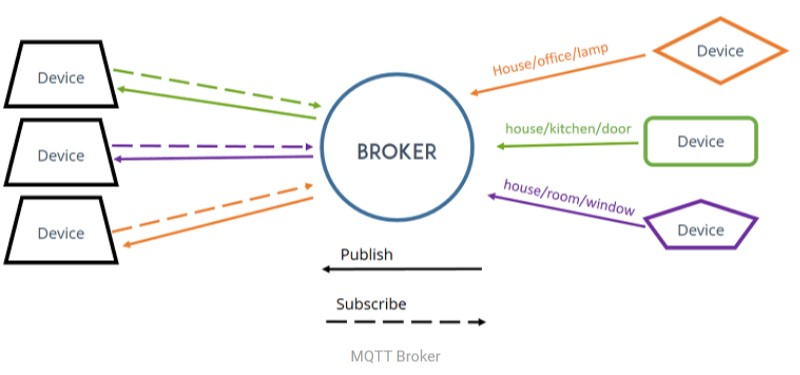
\includegraphics[width=\columnwidth]{Images/1} \\
	\caption{Mô hình MQTT Broker}
	\label{fig:1}
\end{figure}
\subsubsection{Ưu điểm của MQTT Server}
 MQTT mang lại nhiều lợi ích mạnh mẽ cho quy trình:\\
$\indent$ - Chuyển thông tin hiệu quả hơn \\
$\indent$ - Tăng khả năng mở rộng \\
$\indent$ - Giảm đáng kể tiêu thụ băng thông mạng \\
$\indent$ - Giảm tốc độ cập nhật xuống giây \\ 
$\indent$ - Rất phù hợp cho các hoạt động điều khiển \\
$\indent$ - Tối ưu hóa băng thông có sẵn \\
$\indent$ - Chi phí thấp \\
$\indent$ - Rất an toàn với bảo mật dựa trên sự cho phép\\
$\indent$ - Tiết kiệm thời gian phát triển \\
$\indent$ - Giao thức publish/subcribe thu thập dữ liệu được nhiều hơn và sử dụng ít băng thông ít hơn so với giao thức cũ. \\
\newpage
\subsection{Kiến trúc giao tiếp giữa thiết bị, IoT gateway, server và ứng dụng} 
\vspace{0.5cm}

\begin{figure}[tph]
	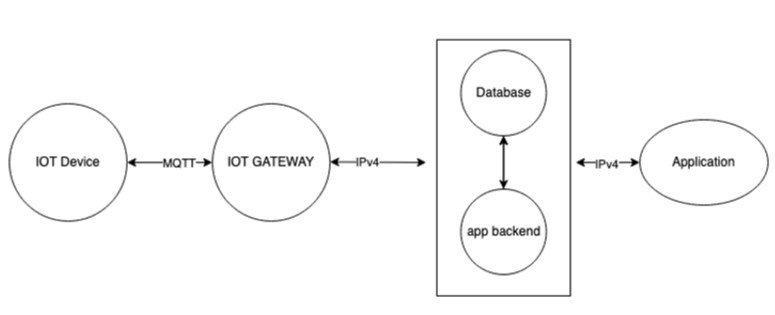
\includegraphics[width=\columnwidth]{Images/IOT}
	\caption{Mô hình kiến trúc hệ thống}
	\label{fig:IOT}
\end{figure} 

$\indent$\textbf{Iot device:} cảm biến, quạt, máy lạnh được kết nối trực tiếp với internet thông qua các cổng kết nối trung gian. \\
$\indent$\textbf{Iot gateway:} nhận data từ mạng truyền thông (Ipv4) chuyển trực tiếp thành data mà các sensor có thể hiểu được theo một giao thức nhất định (ở đây là MQTT)\\
$\indent$\textbf{Server:} Máy chủ lưu trữ dữ liệu và chạy các thuật toán có chức năng xử lý, phân tích dữ liệu để trả về app hoặc gửi xử lý đến IOT Gateway. \\
$\indent$\textbf{Application:} App Android có chức năng nhận diện các tương tác người dùng gửi đến server hoặc nhận dữ liệu trả về từ server hiển thị.\\
\newpage
\section{Mô tả use-case}
\begin{figure}[tph]
	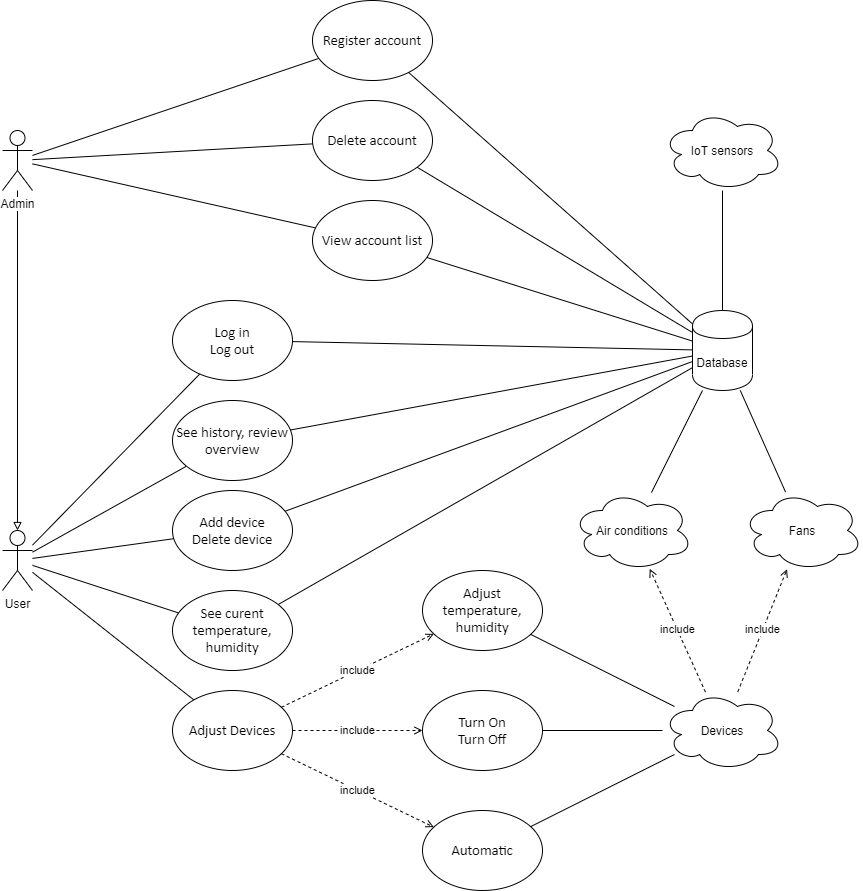
\includegraphics[width=\columnwidth]{Images/Usecase} \\
	\caption{Usecase hệ thống}
	\label{fig:Usecase}
\end{figure} 
\subsection{Xem lịch sử đánh giá tổng quan}
\begin{center}
	\begin{tabular}{|p{4cm}|p{10cm}|}
		\hline
		Tên Usecase & Xem lịch sử đánh giá tổng quan\\ \hline
		Tác nhân & Người dùng (user)\\ \hline
		Mô tả & User xem lịch sử nhiệt độ, độ ẩm qua các ngày, xem đánh giá tổng quan \\ \hline
		
		Điều kiện tiên quyết & Người dùng đang ở trang chủ phần mềm \\ \hline
		Quy trình & \begin{enumerate}
			\item User chọn nút "Xem lịch sử" ở trang chủ
			\item Hê thống hiện ra danh sách các ngày kèm nhiệt độ, độ ẩm trung bình của tòa nhà.
			\item User chọn nút "Đánh giá".
			\item Hệ thống hiện ra biểu đồ nhiệt độ, độ ẩm trung bình và đánh giá mức độ của cả tháng.
		\end{enumerate}\\ \hline
		Ngoại lệ & Ngoại lệ 1: tại bước 2
		nếu không có lịch sử nhiệt độ, độ ẩm của ngày nào thì hệ thống báo "Không có lịch sử" \\ \hline
		Quy trình thay thế & \begin{enumerate}
			\item Quy trình thay thế 1: tại bước 2:
			\subitem User chọn ngày trong ô tìm kiếm.
			\subitem Hệ thống sẽ hiện thông tin lịch sử nhiệt độ, độ ẩm của ngày được chọn
			\item Quy trình thay thế 2: tại bước 3
			\subitem  User chọn hình thức đánh giá (theo tuần, theo tháng)
			\subitem Hệ thống sẽ hiện thông tin lịch sử theo hình thức được lựa chọn
			
		\end{enumerate} \\ \hline
		
	\end{tabular}
\end{center}
\newpage
\subsection{Đăng kí tài khoản }
\begin{center}
	\begin{tabular}{|p{4cm}|p{10cm}|}
		\hline
		Tên Usecase & Đăng kí tài khoản\\ \hline
		Tác nhân & Admin\\ \hline
		Mô tả & Admin đăng kí tài khoản mới cho người sử dụng
		\\ \hline
		Điều kiện tiên quyết & Tài khoản đang sử dụng là admin \\ \hline
		Quy trình & \begin{enumerate}
			\item Admin nhấn vào nút "Danh sách tài khoản".
			\item Hệ thống hiển thị danh sách tài khoản.
			\item Admin nhấn vào nút thêm tài khoản
			\item Hệ thống hiện ra trang đăng kí
			\item Điền thông tin tài khoản và mật khẩu.
			\item Nhấn nút "Tạo tài khoản" để hoàn thành đăng kí.
			\item Hệ thống thông báo "Đăng kí tài khoản thành công!".
			\item Hệ thống trả về trang chủ.
		\end{enumerate}\\ \hline
		Ngoại lệ & \begin{enumerate}
			\item Ngoại lệ 1 tại bước 6: Khi nhập tài khoản đã được tạo thì hệ thống báo “Tài khoản đã tồn tại”.
			\item Ngoại lệ 2 tại bước 6: Khi nhập mật khẩu lần 2 không khớp với mật khẩu lần một thì hệ thống báo “Nhập lại mật khẩu”.
		\end{enumerate} \\ \hline
		Quy trình thay thế &  Không có quy trình thay thế. \\ \hline
		
	\end{tabular}
\end{center}
\subsection{Xóa tài khoản}
\begin{center}
	\begin{tabular}{|p{4cm}|p{10cm}|}
		\hline
		Tên Usecase & Xóa tài khoản\\ \hline
		Tác nhân & Admin\\ \hline
		Mô tả & Admin xóa tài khoản người sử dụng
		\\ \hline
		Điều kiện tiên quyết & Tài khoản đang sử dụng là admin \\ \hline
		Quy trình & \begin{enumerate}
			\item Admin nhấn vào nút "Danh sách tài khoản".
			\item Hệ thống hiển thị danh sách tài khoản và ô tìm kiếm.
			\item Nhập tên tài khoản vào ô tìm kiếm.
			\item Admin nhấn vào nút “Xóa tài khoản” bên phải tên tài khoản.
			\item Hệ thống gửi thông báo xác nhận xóa tài khoản.
			\item Kích vào nút Delete để xóa tài khoản.
		\end{enumerate}\\ \hline
		Ngoại lệ & Ngoại lệ 1 tại bước 3: Tên tài khoản chưa được tạo thì hệ thống thông báo “Tài khoản không tồn tại”
		\\ \hline
		Quy trình thay thế &
		Tại bước 3: Thực hiện chọn tên tài khoản có sẵn ở danh sách bên dưới ô tìm kiếm.
		\\ \hline
		
	\end{tabular}
\end{center}
\subsection{Xem danh sách tài khoản}
\begin{center}
	\begin{tabular}{|p{4cm}|p{10cm}|}
		\hline
		Tên Usecase & Xem danh sách tài khoản.\\ \hline
		Tác nhân & Admin\\ \hline
		Mô tả & Admin xem danh sách các tài khoản.
		\\ \hline
		Điều kiện tiên quyết & Tài khoản đang sử dụng là admin \\ \hline
		Quy trình & \begin{enumerate}
			\item  Admin nhấp vào nút “Xem danh sách tài khoản”
			\item Hệ thống hiện ra danh sách các tài khoản
			
		\end{enumerate}\\ \hline
		Ngoại lệ & Không có ngoại lệ.\\ \hline
		Quy trình thay thế & Không có quy trình thay thế. \\ \hline
		
	\end{tabular}
\end{center}
\subsection{Đăng nhập tài khoản}
\begin{center}
	\begin{tabular}{|p{4cm}|p{10cm}|}
		\hline
		Tên Usecase & Đăng nhập\\ \hline
		Tác nhân & Admin, user\\ \hline
		Mô tả & Admin hoặc người dùng thực hiện đăng nhập vào hệ thống
		\\ \hline
		Điều kiện tiên quyết & Không có điều kiện tiên quyết. \\ \hline
		Quy trình & \begin{enumerate}
			\item Người dùng nhập username, password.
			\item Hệ thống thông báo "Đăng nhập thành công", hiển thị trang chủ.
		\end{enumerate}\\ \hline
		Ngoại lệ & Ngoại lệ tại bước 1: 
		\begin{enumerate} 
			\item Tên tài khoản hoặc mật khẩu không đúng thì hệ thông báo "Sai tên tài khoản hoặc mật khẩu". 
			\item Hệ thống yêu cầu người dùng nhập lại user, password.
		\end{enumerate}\\ \hline
		Quy trình thay thế & Không có quy trình thay thế. \\ \hline
		
	\end{tabular}
\end{center}
\subsection{Đăng xuất tài khoản}
\begin{center}
	\begin{tabular}{|p{4cm}|p{10cm}|}
		\hline
		Tên Usecase & Đăng xuất\\ \hline
		Tác nhân & Admin, user.\\ \hline
		Mô tả & Admin hoặc người dùng thực hiện đăng xuất khỏi hệ thống.
		\\ \hline
		Điều kiện tiên quyết & Đã đăng nhập vào hệ thống \\ \hline
		Quy trình & \begin{enumerate}
			\item  Người dùng nhấn vào nút "Đăng xuất".
			\item Hệ thống xác thực việc đăng xuất.
			\item Sau khi nhấn OK, đăng xuất khỏi hệ thống. Hệ thống quay lại hiển thị trang đăng nhập.
		\end{enumerate}\\ \hline
		Ngoại lệ & Không có ngoại lệ.\\ \hline
		Quy trình thay thế & Không có quy trình thay thế.\\ \hline
		
	\end{tabular}
\end{center}

\subsection{Thêm bớt thiết bị điều khiển}
\begin{center}
	\begin{tabular}{|p{4cm}|p{10cm}|}
		\hline
		Tên Usecase & Thêm bớt thiết bị\\ \hline
		Tác nhân & User \\ \hline
		Mô tả & Thực hiện cập nhật thêm bớt thiết bị vào hệ thống
		\\ \hline
		Điều kiện tiên quyết & \begin{enumerate}
			\item Người dùng phải là user.
		\end{enumerate} \\ \hline
		Quy trình & \begin{enumerate}
			\item Người dùng nhấn "Hiển thị danh sách thiết bị".
			\item Hệ thống hiện ra giao diện chứa danh sách các thiết bị và ô tìm kiếm.
			\item Nhấp vào nút “Add” để thêm thiết bị
			\item Điền thông tin của thiết bị vào các ô tương ứng
			\item Nhấn nút "OK" để thêm hoặc "Cancel" để hủy.
			\item Màn hình trả về các danh sách thiết bị.
		\end{enumerate}\\ \hline
		Ngoại lệ & Không có ngoại lệ. \\ \hline
		Quy trình thay thế & Tại bước 3:
		\begin{enumerate}	
			\item Nhấp chọn thiết bị hoặc tìm ID của thiết bị
			\item Nhấp nút “Delete” và xác nhận để xóa thiết bị
		\end{enumerate}\\ \hline
		
	\end{tabular}
\end{center}

\subsection{Xem độ ẩm, nhiệt độ hiện tại}
\begin{center}
	\begin{tabular}{|p{4cm}|p{10cm}|}
		\hline
		Tên Usecase & Xem độ ẩm, nhiệt độ hiện tại.\\ \hline
		Tác nhân & User \\ \hline
		Mô tả & Người dùng xem nhiệt độ và độ ẩm hiện tại.
		\\ \hline
		Điều kiện tiên quyết & Người dùng phải đăng nhập vào hệ thống. \\ \hline
		Quy trình & Người dùng xem có chỉ số trên ở trang chủ ứng dụng. \\ \hline
		Ngoại lệ & 
		Nếu không có dữ liệu từ sensor thì thông báo “Không có dữ liệu”
		\\ \hline
		Quy trình thay thế & Không có quy trình thay thế. \\ \hline
		
	\end{tabular}
\end{center}

\subsection{Tự điều chỉnh nhiệt độ, độ ẩm}
\begin{center}
	\begin{tabular}{|p{4cm}|p{10cm}|}
		\hline
		Tên Usecase & Điều chỉnh thiết bị.\\ \hline
		Tác nhân & User\\ \hline
		Mô tả &	Tự cài đặt nhiệt độ độ ẩm cho các thiết bị hoạt động
		\\ \hline
		Điều kiện tiên quyết & Tài khoản đang sử dụng là user. \\ \hline
		Quy trình & \begin{enumerate}
			\item  Admin nhấp vào nút "Điều chỉnh thiết bị."
			\item Hệ thống hiện ra danh sách thiết bị.
			\item  Nhấn vào các thiết bị cần điều chỉnh.
			\item Thay đổi các thiết bị theo nhu cầu.
			\item Người dùng nhấn "Hiển thị danh sách thiết bị".
			\item Hệ thống hiển thị danh sách thiết bị.
			\item Người dùng nhấn vào nút “Điều chỉnh thiết bị”
			\item Người dùng chọn thiết bị cần điều chỉnh
			\item Người dùng chọn chế độ tự cài đặt
			\item Người dùng nhập giá trị nhiệt độ và độ ẩm vào các ô tương ứng để bật tắt thiết bị.
			\item Nhấn nút “Áp dụng” để hoàn thành cài đặt.
			\item Hệ thống hiển thị danh sách thiết bị.
			
		\end{enumerate}\\ \hline
		Ngoại lệ & Không có ngoại lệ.\\ \hline
		Quy trình thay thế & Không có quy trình thay thế\\ \hline
		
	\end{tabular}
\end{center}

\subsection{Bật tắt thiết bị}
\begin{center}
	\begin{tabular}{|p{4cm}|p{10cm}|}
		\hline
		Tên Usecase & Bật tắt thiết bị\\ \hline
		Tác nhân & User\\ \hline
		Mô tả & Điều chỉnh chế độ bật tắt cho các thiết bị.
		\\ \hline
		Điều kiện tiên quyết & Tài khoản đang sử dụng là user \\ \hline
		Quy trình & \begin{enumerate}
			\item Hệ thống hiện ra danh sách các thiết bị.
			\item User nhấn vào nút "Điều chỉnh thiết bị".
			\item Chọn thiết bị cần điều chỉnh.
			\item Điều chỉnh bật tắt thiết bị.
		\end{enumerate} \\ \hline
		Ngoại lệ & Không có ngoại lệ. \\ \hline
		Quy trình thay thế & Không có quy trình thay thế. \\ \hline
		
	\end{tabular}
\end{center}
\subsection{Bật chế độ tự điều chỉnh tự động}
\begin{center}
	\begin{tabular}{|p{4cm}|p{10cm}|}
		\hline
		Tên Usecase & Bật chế độ điều chỉnh tự động\\ \hline
		Tác nhân & User\\ \hline
		Mô tả & Bật chế độ cho các thiết bị tự động bật tắt theo cảm biến nhiệt độ, độ ẩm
		\\ \hline
		Điều kiện tiên quyết & Tài khoản đang sử dụng là user \\ \hline
		Quy trình & \begin{enumerate}
			\item Hệ thống hiện ra danh sách các thiết bị.
			\item Người dùng nhấn vào nút “Điều chỉnh thiết bị”
			\item Người dùng chọn thiết bị cần điều chỉnh
			\item Người dùng set chế độ tự động cho thiết bị.
			\item Hệ thống xác nhận "Đã set chế độ tự động cho thiết bị".	
		\end{enumerate} \\ \hline
		Ngoại lệ & Không có ngoại lệ. \\ \hline
		Quy trình thay thế & Không có quy trình thay thế. \\ \hline
		
	\end{tabular}
\end{center}

\section{Tài liệu tham khảo}
\begin{enumerate}
\item https://reactnative.dev/docs/getting-started
\item https://topdev.vn/blog/lap-trinh-app-su-dung-react-native-so-voi-android-ios/
\item https://vi.wikipedia.org/wiki/React\_Native
\item https://reactguide.org/react-native/react-native-overview-and-getting-started.html
\end{enumerate}
\end{document}




\newpage


%%%%%%%%%%%%%%%%%%%%%%%%%%%%%%%%%
\addcontentsline{toc}{section}{Tài liệu tham khảo}
\begin{thebibliography}{99999}



\end{thebibliography}



 
\end{document}

